\chapter{Módszerek}
\pagestyle{headings}

Ezen fejezetben az általam felhasznál anyagokról, eszközökről és alkalmazott módszerekről számolnék be röviden. Törekedve a tömörségre, ahol a módszer rutinszerű, hivatkozom a megfelelő közleményt.

\section{Mikroelektródok készítése}

Laboratóriumi munkám alatt kétféle elektródot használtam. A mérőelektródokat ezek közül saját kezűleg készítettem el a laboratóriumban rendelkezésre álló eszközök és anyagok felhasználásával, előzőleg kidolgozott technikák alapján \cite{{chowdhury1969fabrication},{bretag2017glass}}.
Kiindulásként egy 10 cm hosszúságú, 2 mm külső, 1 mm belső átmérőjű, húzott végű boroszilikát kapillárist használtam (Kwic-Fil$^TM$, World Precision Instruments, Inc., Sarasota, Florida 34240, Amerikai Egyesült Államok). Ezt a kapillárist egy e célból kialakított húzókészülékbe (Sutter Instrument Company, Model P-30, Novato, CA 94949, Amerikai Egyesült Államok) helyeztem, amibe egy kanthalszál (kanthal: alumínium, króm és vas ötvözete) felhevítette és a kapillárist a két végénél fogva egy elektromágnes segítségével széthúzta. A végeredményképp kapott kapilláris nyújtott kúp geometriájú csúccsal rendelkezett, vége pár mikrométer átmérőjű volt. Pontos információm nincs róla, mivel a mérésben nem bírt jelentőséggel, de optikai fénymikroszkóp (Optech LFZ, s/n 220058, Exacta-Optech GmbH, München, Németország) alatt megállapítottam a fentebb említettet, mikor a szabad szemmel nem látható hibák esetlegességét kizártam. Ezután egy $\approx$3 cm hosszúságú, pontosan d=50$\upmu$m átmérőjű ezüstszálat (Ermine Business Park, Huntingdon, England PE29 6WR) helyeztem el a mikroelektródba, majd töltőoldatként 0,1 M-os KCl- oldatot (Sigma-Aldrich Corp.) használtam. Feltöltése során egy főzőpohárba öntöttem a KCl-oldatot és ebbe állítottam a mikróelektródot. Néhány óra elteltével a kapillárishatásnak köszönhetően beszivárgott az oldat és elkészült a mikroméretű referencia elektród (\ref{fig:electrode}. ábra).

\begin{figure}
\centering

\includegraphics[width=0.5\textwidth]{img/electrode.eps}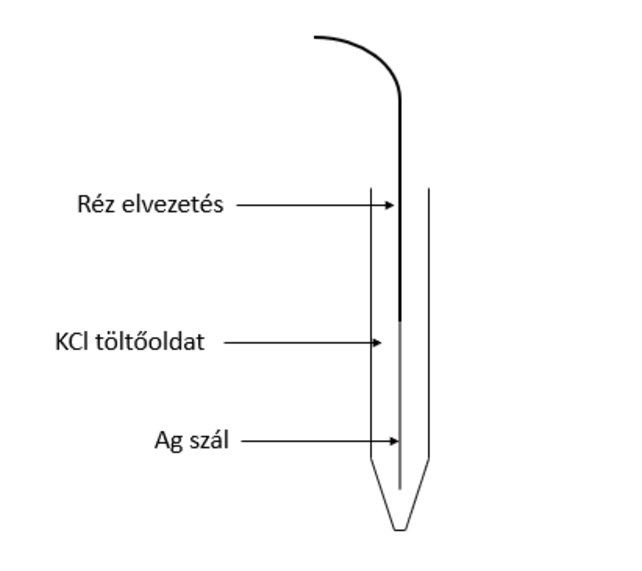
\includegraphics[width=0.5\textwidth]{img/electrode1.eps}

\caption{Az általam készített mikroméretű referencia elektród és sematikus ábrája}
\label{fig:electrode}
\end{figure}

\section{Céltárgyak}

Laboratóriumi munkám során kétféle céltárgyat alkalmaztam: egy állandó rendszerű grafit céltárgyat és egy vas-cink galvánpárt. Ez utóbbi a galvanikus korrózió jellemzésére tökéletesen megfelelő volt. Mindkét céltárgy epoxi gyantába volt öntve, így a grafit és fémminta egy meghatározott része érintkezett az oldattal. Az epoxi gyanta alsó részén rézdrótok által volt megoldva az elektromos elvezetés. Minden mérés előtt és után, a céltárgyak felületét políroztam, csiszolópapír segítségével. Ezután, hogy a cellát létrehozzam és oldatot öntsek a felületére a mintának, hézagmentesen körbetekertem átlátszó ragasztószalaggal, úgy hogy körülbelül fél centiméterrel magasabban legyen a céltárgy felületétől. Szintezettségét is be kellett állítanom a céltárgyak felszínének minden mérés előtt, ehhez egy buborékos vízszintezőt használtam. Így a pásztázás síkja párhuzamos volt a céltárgy X-Y síkjával. A cella létrehozásához szükséges oldatként a laboratóriumban található desztilálló készülék (Elix® Essential 10 Water Purification System, Milli-Q, Progard® TS2, PR0G0T0S2) által előállított desztillált vizet használtam, melynek vezetése 0,067 $\upmu$A/cm volt. Ez utóbbi adatot a készülék szolgáltatta szintén.

\section{Mikroszkóp és a mérőprogram}

A mérésekhez egy, a tanszéken a közelmúltban épített pásztázó elektrokémiai mikroszkópot (Eppendorf MIM4 Micromanipulator), valamint egy nagy impedanciájú mérőműszert (eDAQ QUAD MF isoPod 452) használtam, mely utóbbit  eDAQ Pod-Vu nevezetű program vezérelt. Kétféle pásztázási algoritmust használtam, horizontális, a minta felületének síkjával párhuzamos 2D pásztázást, és a minta felületének síkjára merőleges 2D pásztázást. Az X és Y irányú lépésköz 100 $\upmu$m volt minden esetben. A teljes pásztázott terület a mintától függött, melyről a mérési eredmények ismertetése során írok részletesen. A mikroelektród mozgatási sebessége két szomszédos mérési pont között 1000 $\upmu$m/s volt. Minden egyes mérés előtt 0.2 s várakozási időt adtam meg, hogy a mozgatást követően egy közel egyensúlyi, stabil potenciál érték kialakulhasson.  

Mivel az elektromos mező Z irány komponenséhez vertikális potenciálkülönbség mérésekre van szükség, a horizontális pásztázásokat kétszer végeztem el, bizonyos Z irány eltolással, melyet az egyes mérések bemutatásánál adok meg.

A mérések előtt a Z referencia koordinátát a következő módon állítottam be. A poteniometriás méréseknél ismeretes, hogy a Z koordináta beállítása nehézségekbe ütközik. Ezt a következőképp oldottam meg: miután elhelyeztem a mikroméretű referencia elektródot a mikroszkóp foglalatába, elkezdtem közelíteni az adott céltárgy felületéhez, annak a galvánpár közötti középpontja felé. Mikor szemmel láthatólag közel volt a felülethez, kis mértékben közelítettem, majd mozgattam minimálisan az elektródot, hogy a felülettel együtt mozog-e. Ha nem még közelítettem, hogy ütközésig érjen hozzá. Amikor ezt elértem, 0 mikrométernek tekintettem ezt, és innentől számítva adtam meg a programnak, hogy hány mikrométerrel a céltárgy felett mozogjon Z irányban. Így, mint említettem korábban, a pásztázási terület középpontjában volt az elektród. Viszont a program meanderezve haladt, jobbról balra, majd ugrott egyet a következő pásztázási vonal jobb oldalára újra.  Emiatt a teljes pásztázási terület ½ értékével léptem, tehát X/2 és Y/2 értékkel, hogy eljussak a mérés kezdőpontjába. 

\section{Mérések kiértékelése}

A mérések eredményeképp kapott potenciáltértképeket először deriválnom kellett, hely szerint. Az dat kiterjesztésű adatfájlokat egyenként importáltam a Qti Plot nevű programba, egy táblázatba, ami X-Y-E oszlopokból állt. X és Y oszlopok tartalmazták a mérések lépéseit, E pedig a mért potenciálérték. Ezután a potenciálértékek oszlopát mátrixszá alakítottam, a méréseknek megfelelő oszlop és sor számúra. Grafit minta esetében a vertikálisnál 51 oszlopos 11 soros, horizontális mérésnél két darab 41 oszlopos és 31 soros mátrixot kaptam. A vas-cink céltárgynál vertikális mérésnél 31 oszlopos és 11 soros az anód és katód esetén is, horizontálisan pedig két-két darab az anód és katód oldaláról, amik 31 oszlopot és 21 sort tartalmaztak. 

Az így kapott mátrixokat Excelbe importáltam és X-Y irányba kiszámoltam a cellák közti különbséget. Vagyis a táblázat egy adott potenciálértéke alatti és feletti, illetve két oldali értékek különbségét. X komponens esetén két 0 értékeket tartalmazó oszlopot, Y komponens esetén pedig két 0 értékeket tartalmazó sort kellett beszúrnom, hogy megtartsam az eredeti mátrix paramétereit. Ezt elvégeztem az összes horizontális és vertikális mérési eredményen. Így megkaptam az X és Y komponenseket, melyeket bevittem mátrixként ismét a Qti Plot programba. Szükségem volt még egy Z komponensre is, ezt a horizontális adatokból számítottam ki Excelbe, méghozzá úgy, hogy a két mérés magassága szerinti köztes értéket számoltam ki. Példának véve a grafit céltárgyat, ahol a horizontális mérések 100 mikrométer és 300 mikrométer magasba készítettem. A keresett Z komponens tehát 200 mikrométer magasba volt, amit egyszerűen megkaptam úgy, hogy a 300 mikrométeres mátrix értékeiből kivontam a 100 mikrométeres értékeket. Az összes horizontális esetében így jártam el, majd ezen mátrixokat is importáltam a Qti Plot-ba mátrixként. Ily módon megkaptam az X-Y-Z komponensek mátrixát.

Következő lépésben a mátrixokat visszaalakítottam táblázatos formába, mely három oszlopos volt, az első kettő a mérés paraméterei, a harmadik pedig a számolt komponensek külön-külön táblázatban. Minden méréshez elkészítettem hasonló módon ezt a X-Y-Z komponenst tartalmazó három táblázatot. Ezekből a táblázatokból pedig az X-Y-Z számolt komponenseket, vagyis a harmadik oszlopot importáltam az eredeti táblázatba, így kaptam összesen hat oszlopot. Illetve a horizontális pásztázások esetén be kellett szúrnom még egy hetedik oszlopot, ami csupa 0 értékeket tartalmazott. Ez a Gnuplot-al való ábrázolásomhoz volt szükséges, mivel a programnak a 3D-os ábrázoláshoz meg kellett adnom egy Z paramétert is az X és Y mellett. 

Hogy az elektromos mező értékét megkapjam, a mértékegységek figyelembevételével, megszoroztam a számolt komponenseket (vertikális esetben két oszlopot, horizontálisnál pedig hármat) 100-al, mivel $\upmu$S-el számoltam. Az áramsűrűség ábrázolásához ezeket az oszlopokat még a víz fajlagos vezetőképességével is meg kellett szoroznom. Gnuplot ábrázoláshoz a Z komponens oszlopainak áramértékét le kellett nulláznom, mivel nem valós értékeket mutattak. Ez annak tulajdonítható, hogy a pásztázás területének szélein epoxi volt, és a mérés ideje alatt az oldatban változott a potenciálérték. Az elektromos mező esetében hét oszlopot ábrázoltam, az áramsűrűségnél hármat, a Z irány komponens szerint.
